\begin{SingleSpace}
\chapter{Realistic Modelling of Lava Planets}\label{ch:clouds-lava-planets}
\vspace{0.5cm}
% \chapterprecishere{``One face is forever sunlit, and one forever dark, and only the planet's slow liberation gives the twilight zone a semblance of seasons.''\par\raggedleft--- \textup{Stanley G. Weinbaum}, The Lotus Eaters}
\end{SingleSpace}
\vspace{0.5cm}





% 0 -- LEAD-IN PARAGRAPHS

%START ELEMENT




%FRAMING TEXT

In this chapter, I will follow up the idealised model of 55 Cancri e in Chapter \ref{ch:linking-climate-55cnce} with a more realistic and stable GCM including realistic gaseous absorption and cloud formation.

The simulations in Chapter \ref{ch:linking-climate-55cnce} were highly idealised and sometimes unstable. A GCM that represented the radiative transfer in the atmosphere more realistically would be vital to better model the global circulation, as well as to simulate the observed \SI{4.5}{\micro\metre} phase curve more accurately. A more stable GCM would provide more confidence in the results.

In this chapter, I will introduce the updated version of Exo-FMS on a cubed-sphere grid (described in more detail in Appendix X), focusing on its improved stability, the Socrates radiative transfer module, and the DIHRT cloud model.

I will reproduce some of the simulations from Chapter \ref{ch:linking-climate-55cnce}, and show that the new cubed-sphere version of Exo-FMS qualitatively matches the results of the previous latitude-longitude version. I will then discuss some example simulations using the correlated-k radiative transfer module Socrates, and will show that the global circulation is largely the same as in the grey-gas case. Next, I will simulate the observed Spitzer phase curve using a higher resolution calculation, and will relate this to the conribution function. Finally, I will show the results of simulations with the cloud model DIHRT.

I will show that the grey-gas model represents the global circulation of an atmosphere with more realistic radiative transfer well, in most cases.

I will shows that clouds X.

I will argue that the grey-gas model is sufficient to compare to observations.

%SIGNPOSTS


%SUMMARISE CONCLUSIONS




%%%%%%%%%%%%%%%%%%%%%%%%%%%%%%%%%%%%
%SECTION 1 --
\section{Modelling}


%SUBSECTION --
\subsection{Cubed-Sphere Dynamical Core}

The GCM simulations in Section \ref{ch:linking-climate-55cnce} were sometimes unstable due to unphysical instabilities originating at the poles of the planet. The version of Exo-FMS used in that chapter was on a latitude-longitude grid, where the grid size becomes very small at the poles. This can lead to violation of the CFL condition, which can cause the model to crash.

For the GCM simulations in this section, I developed a new version of Exo-FMS based on an updated version of the GFDL finite-volume dynamical core, on a cubed-sphere grid rather than a latitude-longitude grid. This grid has approximately the same grid scale everywhere, so there is no problem at the poles and the model is much more stable. Updating Exo-FMS to use this dynamical core involved producing a new unified interface between all the physical modules and the core, updating the modules to function on a cubed-sphere grid, and producing utilities to run the model and regrid its output. Appendix X discusses the new model in more detail.


%SUBSECTION --
\subsection{SOCRATES Radiative Transfer}

To represent the effect of clouds accurately, we needed a more sophisticated radiative transfer scheme than the semi-grey scheme used in previous chapters. We coupled the correlated-k radiative transfer code SOCRATES to Exo-FMS \citep{Edwards1996socrates}. See Appendix X for more details.

We used a ``spectral file'' from REF, containing absorption data for X. We only focused on the effect of X, so all the other absorbers were always zero.

%SUBSECTION --
\subsection{DIHRT Dynamical Clouds}

%SECTION CONCLUSIONS

%%%%%%%%%%%%%%%%%%%%%%%%%%%%%%%%%%%%
%SECTION 2 --
\section{Control Tests -- H2 and N2}


%SUBSECTION --
\subsection{Circulation Results}

I ran two tests in the new model with the same parameters as Tests X and X in Chapter X but with the semi-grey radiative transfer replaced by the correlated-k Socrates module.

The spectral file was X

Test A is H2 10 bar with 0.1 CO
Test B is N2 10 bar with 0.1 CO


%Test C is H2 10 bar with 0.1 CO

Figure X shows temperature map and zonal wind

The results are similar to grey-gas.

\begin{figure}
  \centering
  \begin{subfigure}[t]{0.49\textwidth}
    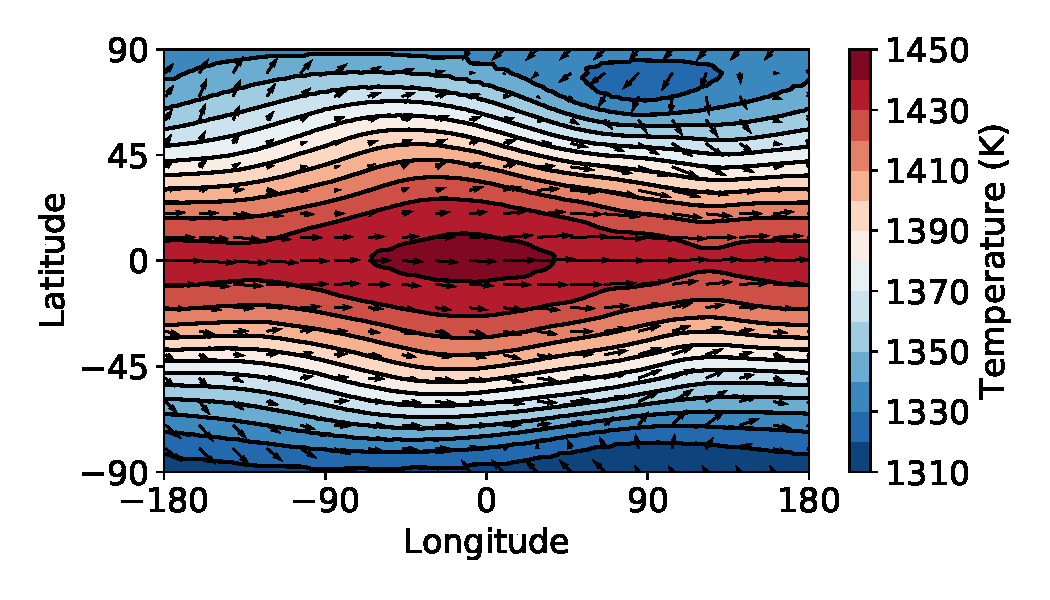
\includegraphics[width=\textwidth]{figures/soc-lava-planets/h2-soc-temp.pdf}
    \caption{10 bar H$_{2}$ atmosphere.}\label{fig:soc-temp-h2}
  \end{subfigure}
  %
  \begin{subfigure}[t]{0.49\textwidth}
    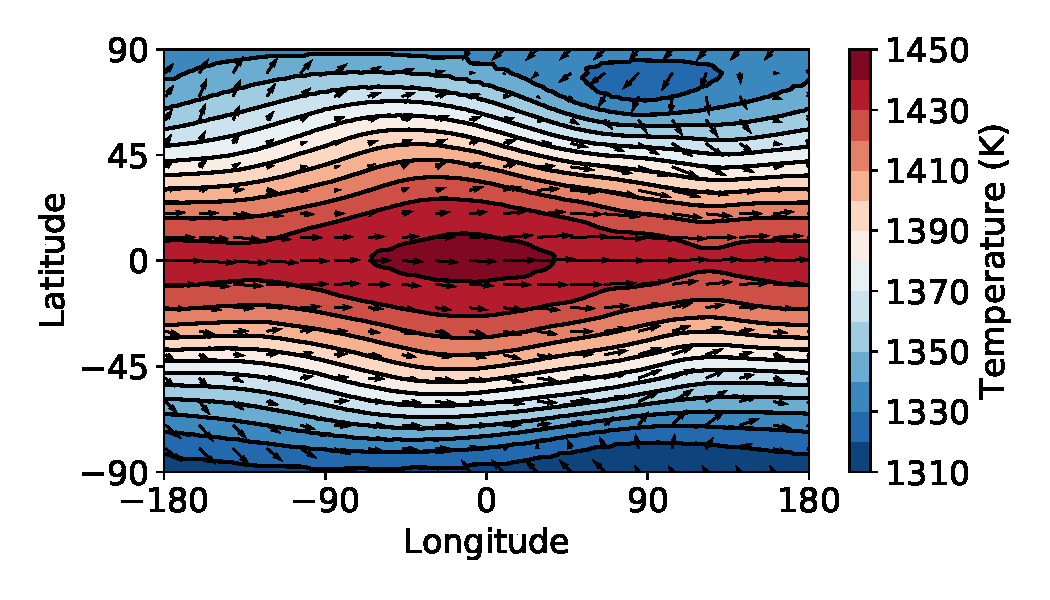
\includegraphics[width=\textwidth]{figures/soc-lava-planets/h2-soc-temp.pdf}
    \caption{10 bar N$_{2}$ atmosphere.}\label{fig:soc-temp-n2}
  \end{subfigure}
  \caption{Global temperature maps of the simulations with $1\%$ CO, at the X pressure level. }
  \label{fig:soc-temp}
\end{figure}

\begin{figure}
  \centering
  \begin{subfigure}[t]{0.49\textwidth}
    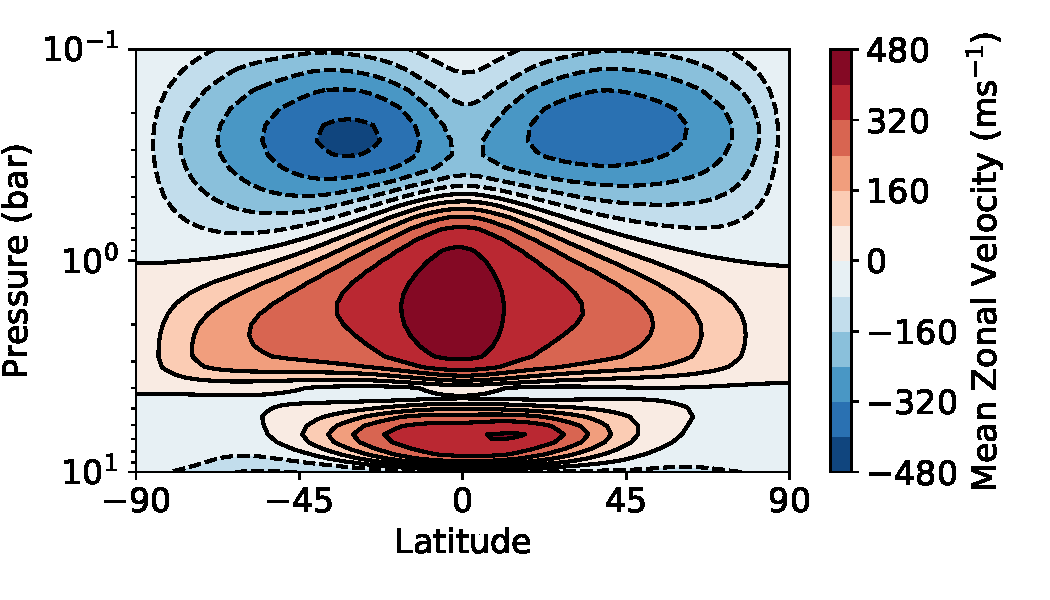
\includegraphics[width=\textwidth]{figures/soc-lava-planets/h2-soc-zonal-u.pdf}
    \caption{10 bar H$_{2}$ atmosphere.}\label{fig:soc-zonal-u-h2}
  \end{subfigure}
  %
  \begin{subfigure}[t]{0.49\textwidth}
    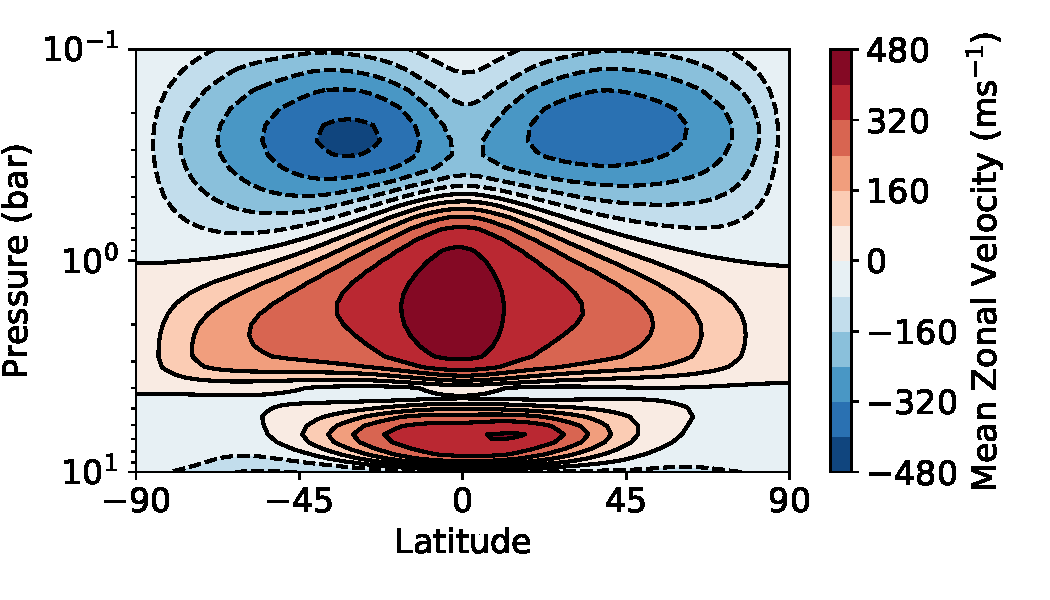
\includegraphics[width=\textwidth]{figures/soc-lava-planets/h2-soc-zonal-u.pdf}
    \caption{10 bar N$_{2}$ atmosphere.}\label{fig:soc-zonal-u-n2}
  \end{subfigure}
  \caption{Zonal-mean zonal wind of the simulations with $1\%$ CO.}
  \label{fig:soc-zonal-u}
\end{figure}

\begin{figure}
  \centering
  \begin{subfigure}[t]{0.49\textwidth}
    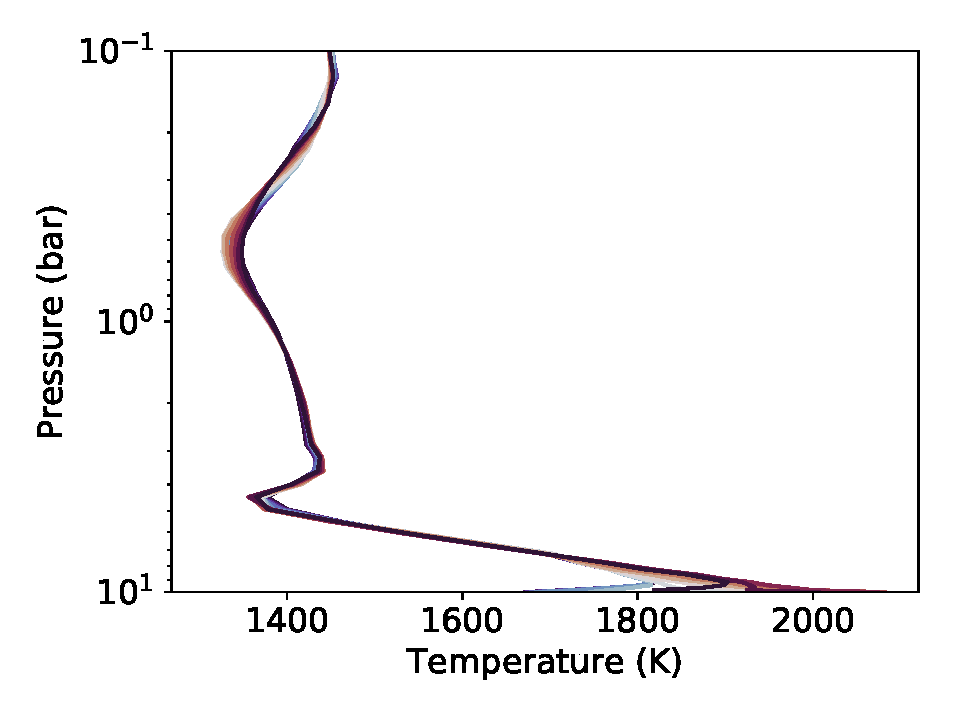
\includegraphics[width=\textwidth]{figures/soc-lava-planets/h2-soc-tp.pdf}
    \caption{10 bar H$_{2}$ atmosphere.}\label{fig:soc-tp-h2}
  \end{subfigure}
  %
  \begin{subfigure}[t]{0.49\textwidth}
    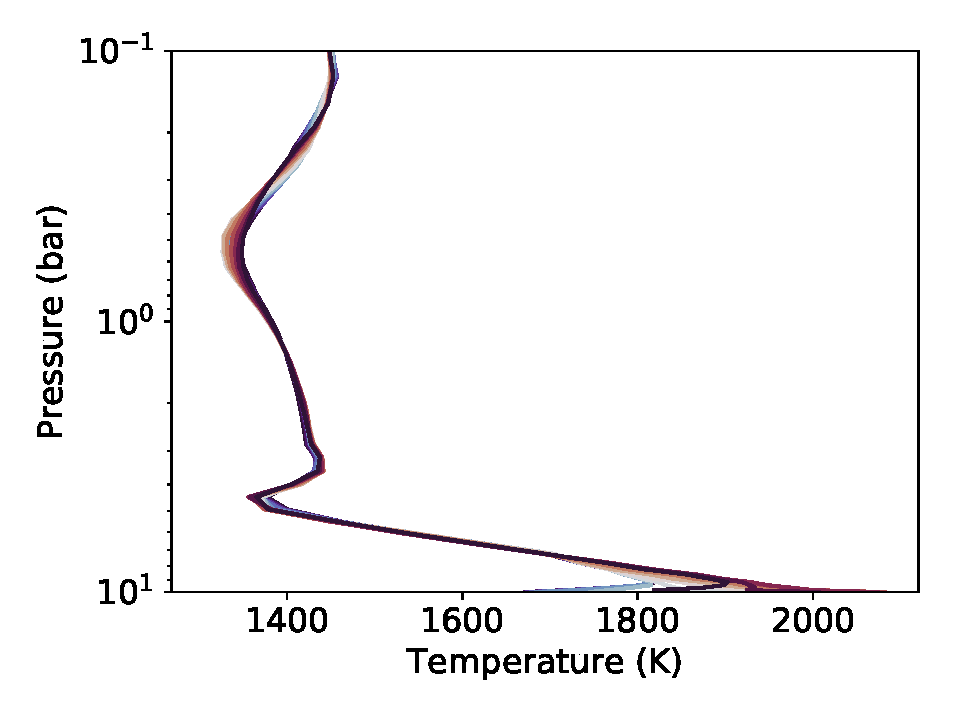
\includegraphics[width=\textwidth]{figures/soc-lava-planets/h2-soc-tp.pdf}
    \caption{10 bar N$_{2}$ atmosphere.}\label{fig:soc-tp-n2}
  \end{subfigure}
  \caption{Temperature profiles of the simulations with $1\%$ CO.}
  \label{fig:soc-tp}
\end{figure}


% I ran the same Socrates tests with SW absorption
%
% Test 5 is N2 10 bar with X CO2?
%
% Test 6 is H2 10 bar with X CO2?
%
% SW absorption can change results.
%
%
% Difficult to do ``inverse'' modelling with so many parameters and unknowns. But, constraints from other measurements can help, e.g. Hot Jupiters we know bulk composition, likely absorbers etc.

%SUBSECTION --
\subsection{Thermal Emission}

The effect of atmospheric opacity on phase curve.

Figure X shows the spectral OLR for Socrates test H2, N2, and H2N2. The Spitzer bandpass is marked. The wavelengths of the phase curves in Figure X are marked, and were chosen to show regions of low, mediu, and high opacity.

Figure X shows phase curves for the Socrates test H2, N2, and H2N2, at the wavelengths marked in Figure X.

The CO has three main absorption features.

The H2 test

The N2 test

\begin{figure}
  \centering
  \begin{subfigure}[t]{0.49\textwidth}
    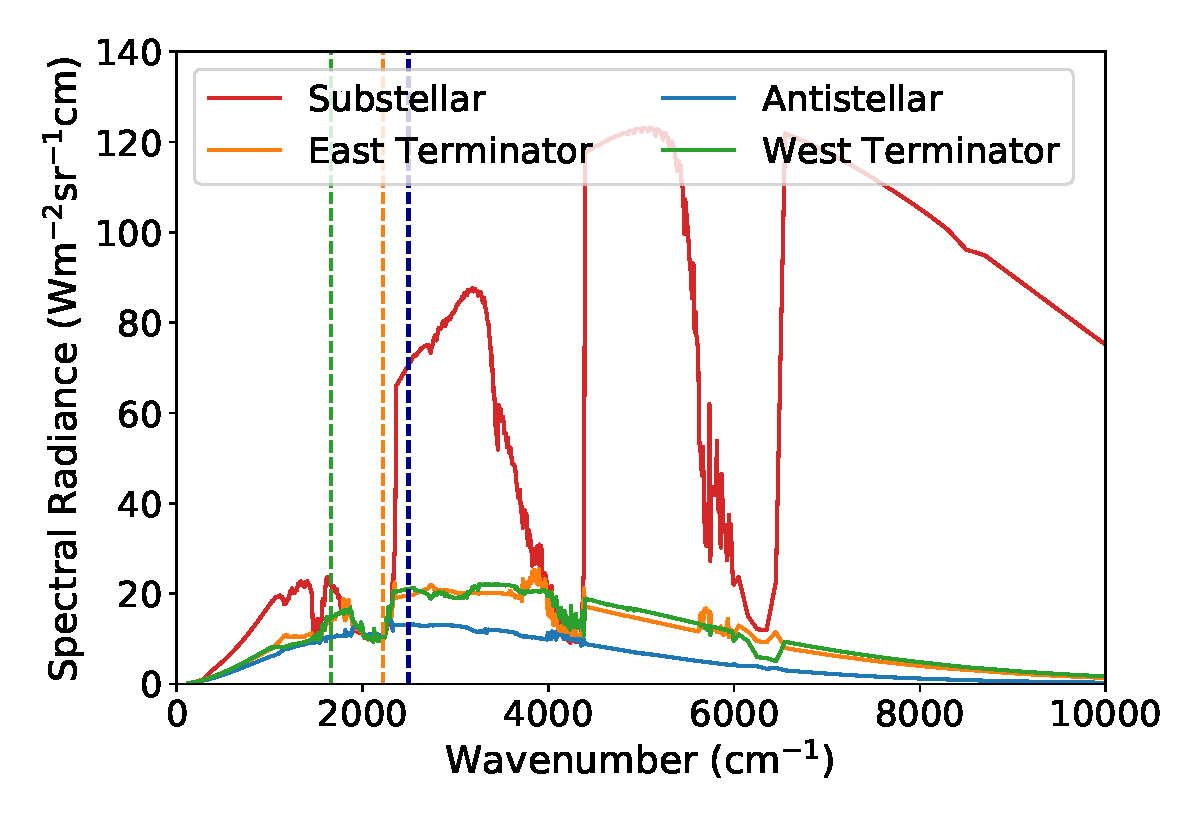
\includegraphics[width=\textwidth]{figures/soc-lava-planets/n2-spec-olr.pdf}
    \caption{10 bar H$_{2}$ atmosphere.}\label{fig:soc-tp-h2}
  \end{subfigure}
  %
  \begin{subfigure}[t]{0.49\textwidth}
    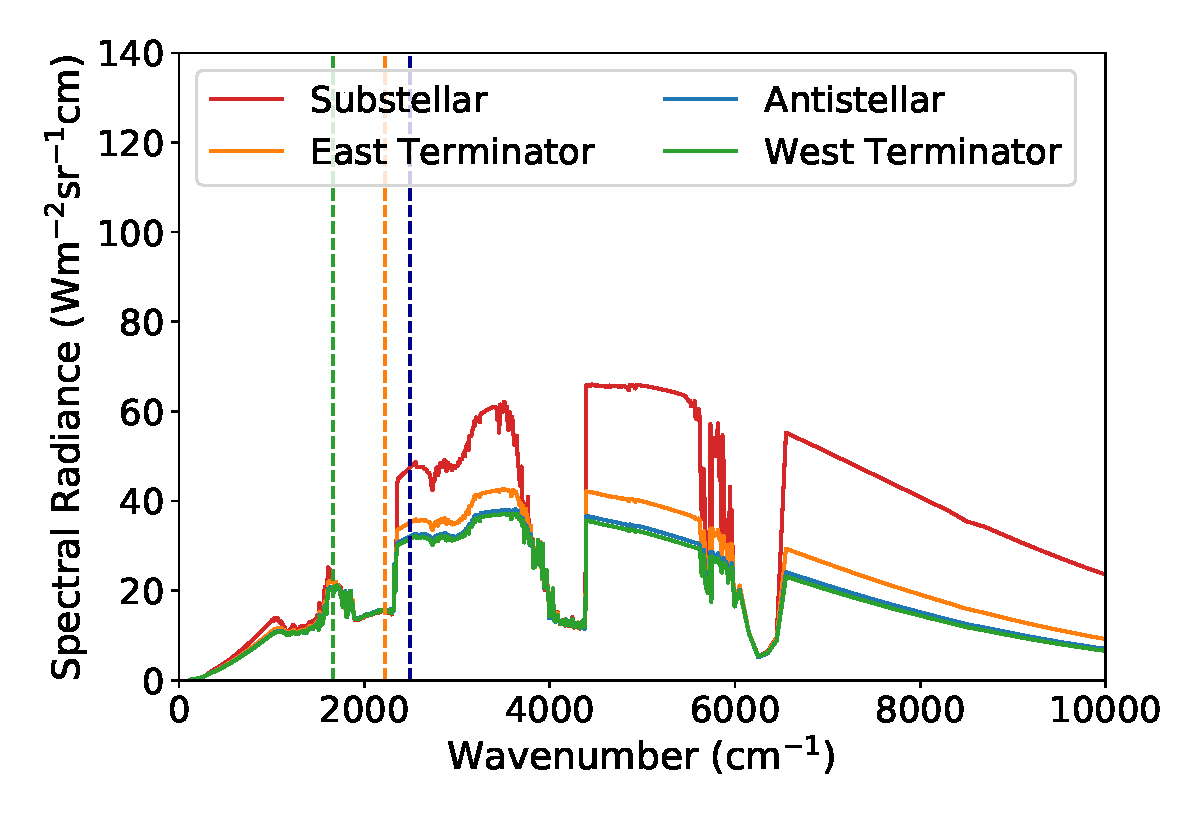
\includegraphics[width=\textwidth]{figures/soc-lava-planets/h2-spec-olr.pdf}
    \caption{10 bar N$_{2}$ atmosphere.}\label{fig:soc-tp-n2}
  \end{subfigure}
  \caption{Temperature profiles of the simulations with $1\%$ CO.}
  \label{fig:soc-tp}
\end{figure}

\begin{figure}
  \centering
  \begin{subfigure}[t]{0.49\textwidth}
    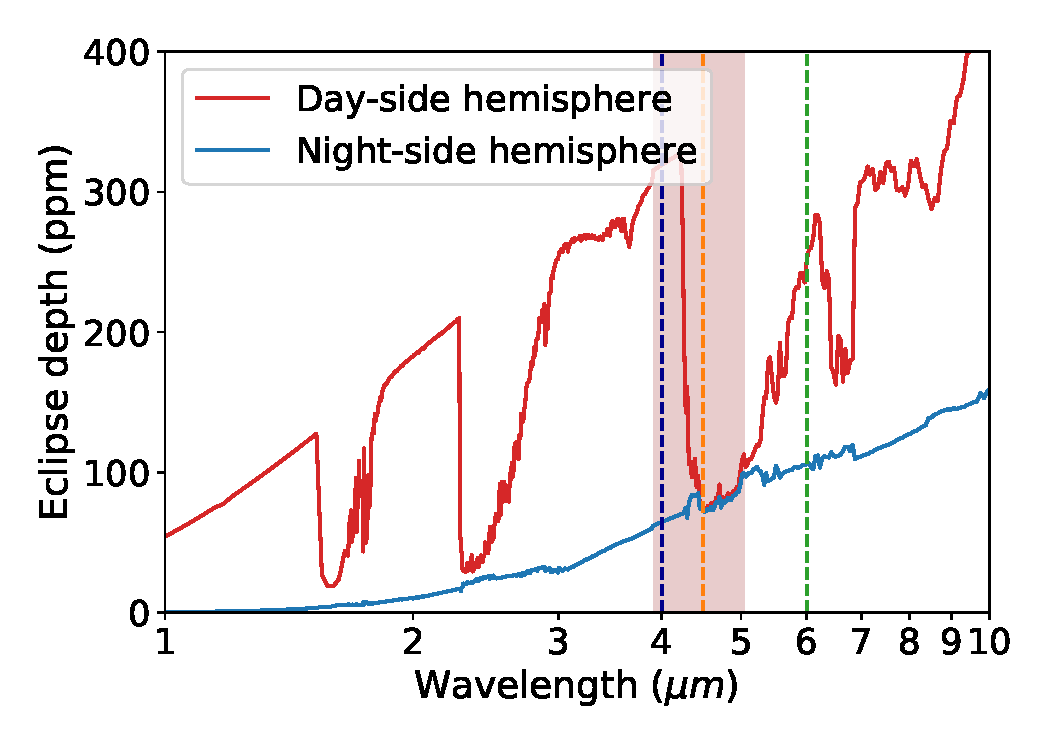
\includegraphics[width=\textwidth]{figures/soc-lava-planets/n2-emission-spec.pdf}
    \caption{10 bar H$_{2}$ atmosphere.}\label{fig:soc-tp-h2}
  \end{subfigure}
  %
  \begin{subfigure}[t]{0.49\textwidth}
    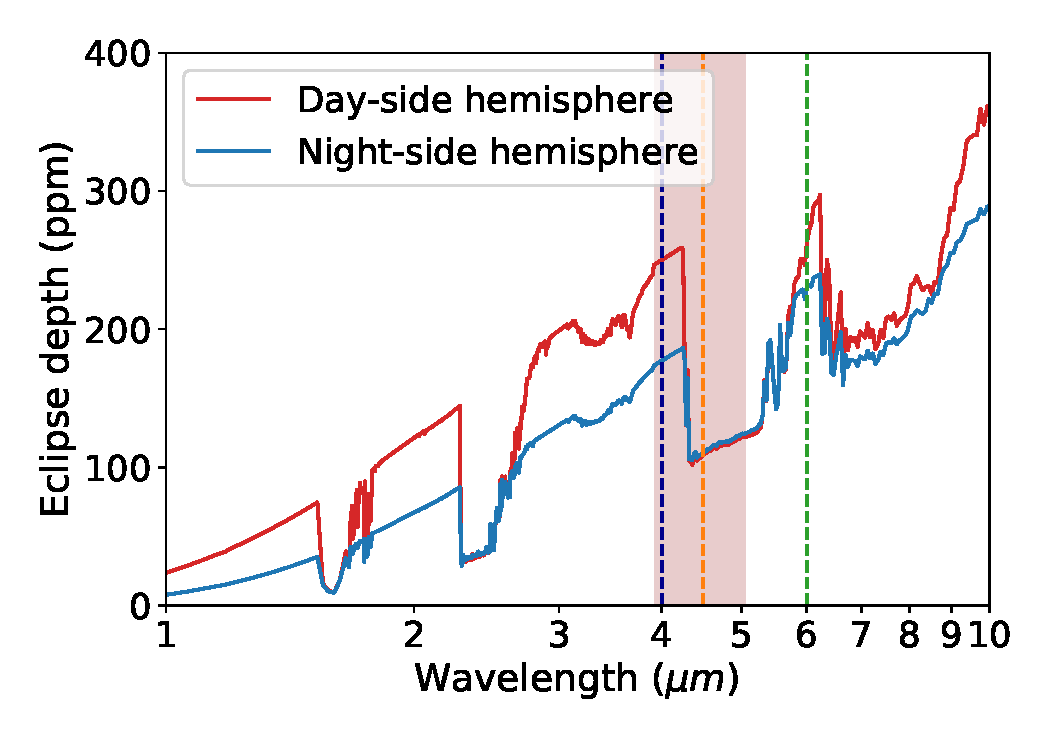
\includegraphics[width=\textwidth]{figures/soc-lava-planets/h2-emission-spec.pdf}
    \caption{10 bar N$_{2}$ atmosphere.}\label{fig:soc-tp-n2}
  \end{subfigure}
  \caption{Temperature profiles of the simulations with $1\%$ CO.}
  \label{fig:soc-tp}
\end{figure}



\begin{figure}
  \centering
  \begin{subfigure}[t]{0.49\textwidth}
    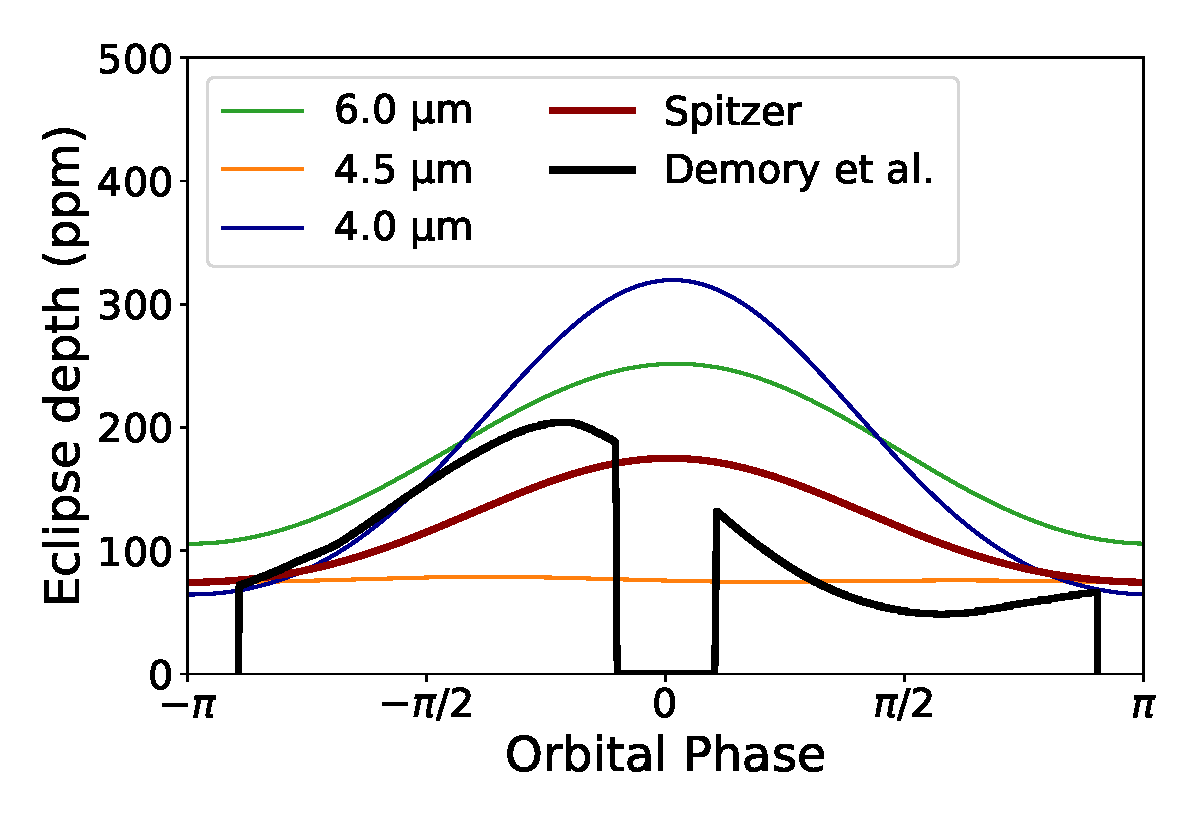
\includegraphics[width=\textwidth]{figures/soc-lava-planets/n2-spec-pc.pdf}
    \caption{10 bar H$_{2}$ atmosphere.}\label{fig:soc-tp-h2}
  \end{subfigure}
  %
  \begin{subfigure}[t]{0.49\textwidth}
    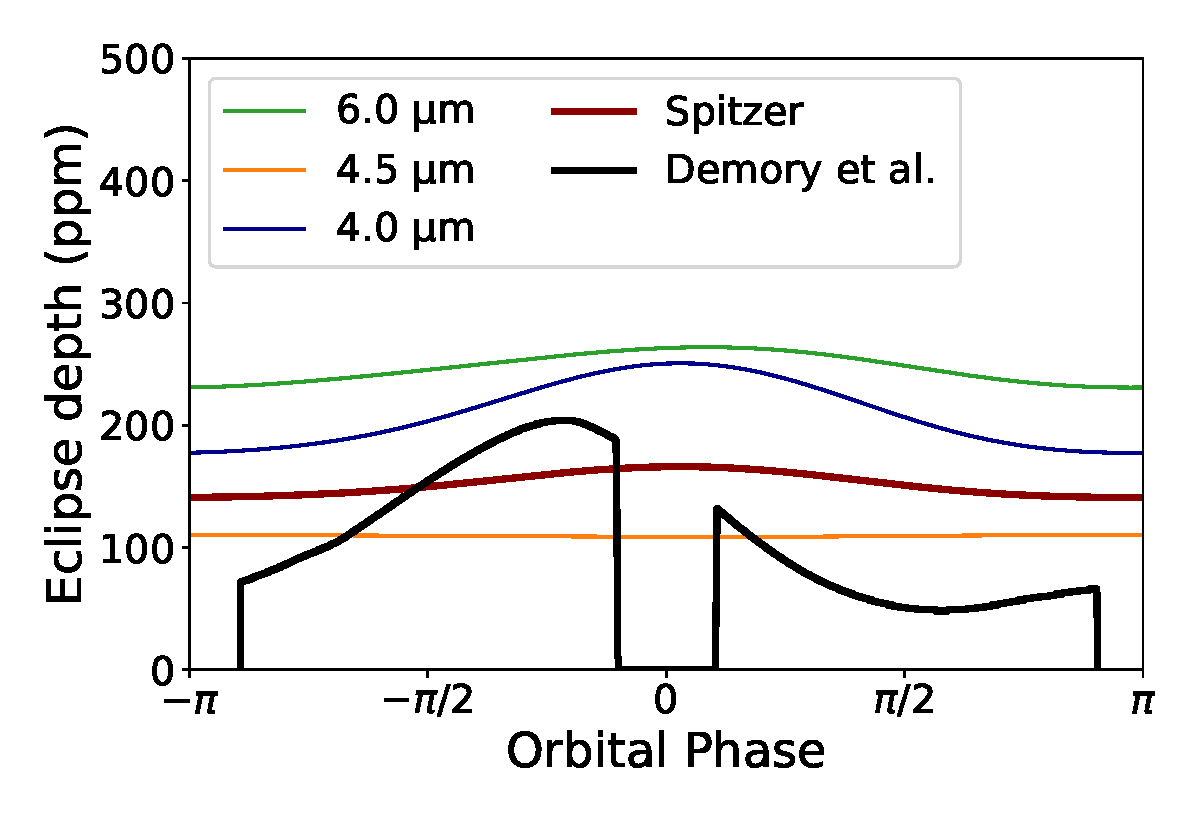
\includegraphics[width=\textwidth]{figures/soc-lava-planets/h2-spec-pc.pdf}
    \caption{10 bar N$_{2}$ atmosphere.}\label{fig:soc-tp-n2}
  \end{subfigure}
  \caption{Temperature profiles of the simulations with $1\%$ CO.}
  \label{fig:soc-tp}
\end{figure}

%SUBSECTION --
\subsection{Contribution Function}

Figure X shows the Socrates contribution function at wavelength X

\begin{figure}
  \centering
  \begin{subfigure}[t]{0.49\textwidth}
    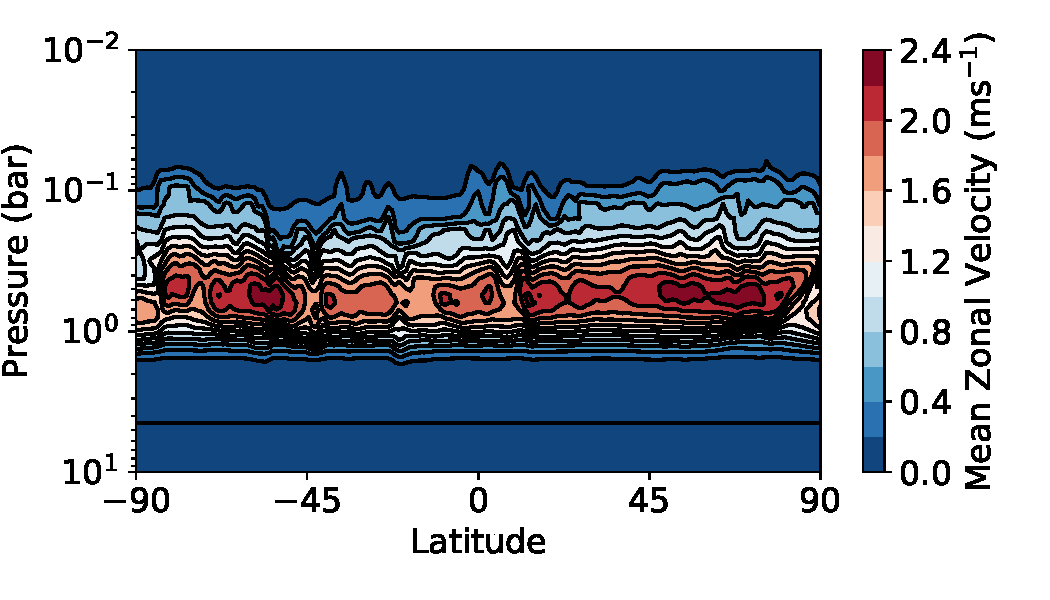
\includegraphics[width=\textwidth]{figures/soc-lava-planets/h2-cf.pdf}
    \caption{10 bar H$_{2}$ atmosphere.}\label{fig:soc-tp-h2}
  \end{subfigure}
  %
  \begin{subfigure}[t]{0.49\textwidth}
    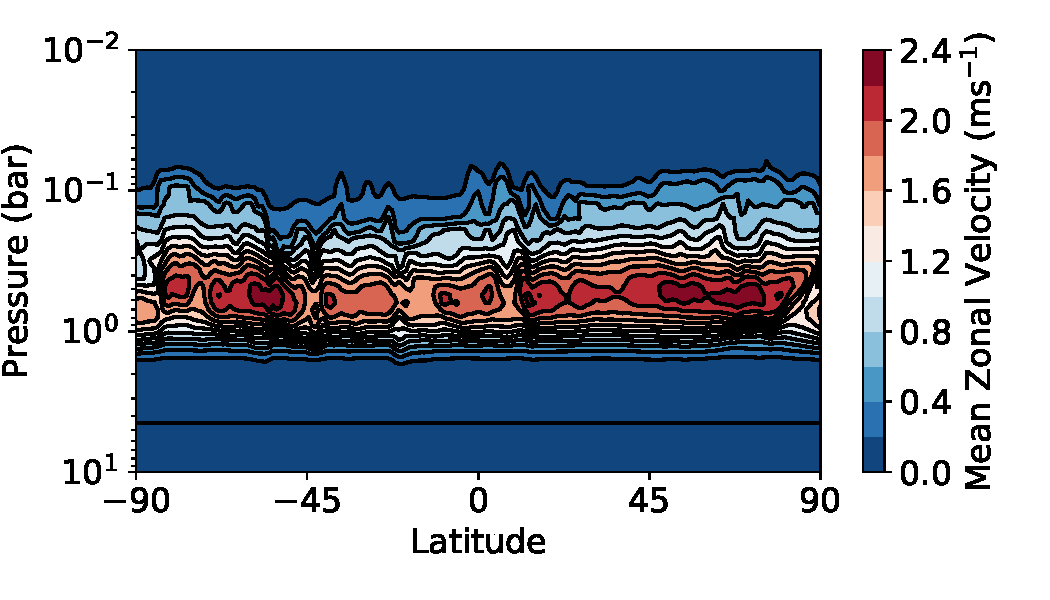
\includegraphics[width=\textwidth]{figures/soc-lava-planets/h2-cf.pdf}
    \caption{10 bar N$_{2}$ atmosphere.}\label{fig:soc-tp-n2}
  \end{subfigure}
  \caption{Temperature profiles of the simulations with $1\%$ CO.}
  \label{fig:soc-tp}
\end{figure}


\section{Best-Fit Test}

H2N2 test

%SUBSECTION --
\subsection{Circulation Results}

Figure X shows the temperature map

Figure X shows the zonal wind

FIgure X shows the temperature profiles

%SUBSECTION --
\subsection{Thermal Emission}

Figure X shows the emission spectrum

Figure X shows the phase curves corresponding to the highlighted wavelengths

%SUBSECTION --
\subsection{Spitzer bandpass phase curves}

Figure X shows phase curves for the Socrates test H2, N2 and H2N2 in the \SI{4.5}{\micro\metre} Spitzer bandpass.

The 4.5 Spitzer bandpass from 4 to 5 would cover the transparent and opaque regions, spanning in and out of the feature. This could X.


\begin{figure}
  \centering
    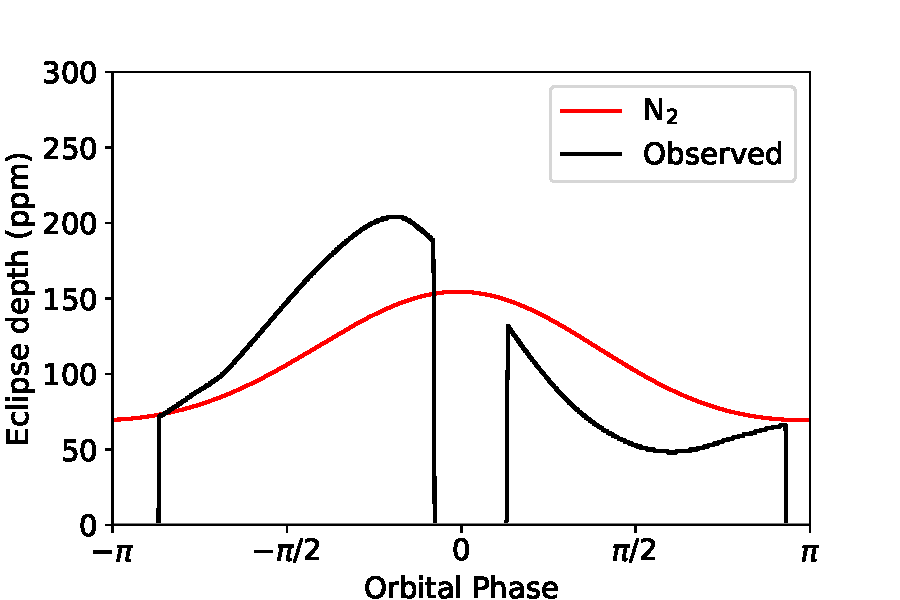
\includegraphics[width=0.49\textwidth]{figures/soc-lava-planets/spitzer-pc.pdf}
    \caption{10 bar N$_{2}$ atmosphere.}\label{fig:soc-tp-n2}
\end{figure}



%SECTION CONCLUSIONS


%%%%%%%%%%%%%%%%%%%%%%%%%%%%%%%%%%%%
%SECTION 3 --
\section{Cloudy Simulations}


%SUBSECTION --
\subsection{Pure CO Atmosphere}

Figure X shows temperature map and zonal wind




%SECTION CONCLUSIONS

%%%%%%%%%%%%%%%%%%%%%%%%%%%%%%%%%%%%
%SECTION 5 --
\section{Discussion}

%SUBSECTION --
\subsection{Analysing 55 Cancri e phase curve}

Predict scaling of jets on 55 Cancri e/lava planets.

Predict linear shallow-water hot-spot shift and day-night contrast.

Predict what similar planets would do at different temperatures.

Explain how this dynamical theory and models could be applied to Hot Jupiters, other tidally locked planets.

%SUBSECTION --
\subsection{Analysing Hot Jupiter phase curve}

Scaling relations

%SECTION CONCLUSIONS

%%%%%%%%%%%%%%%%%%%%%%%%%%%%%%%%%%%%
%CONCLUSIONS
\section{Conclusions}

%RESTATE SECTION CONCLUSIONS

%OPEN OUT CONCLUSIONS


% \bibliographystyle{unsrtnat}
% \bibliography{../references.bib}
